\section{XQuery}
\label{sect:theory:xquery}

XQuery is a query language developed by the XML Query working group of W3C.
Version 1.0\cite{w3c00} became a W3C Recommendation January 2007. It was
designed as a response to an emerging task: to intelligently express queries in
the increasing amounts of information stored, exchanged and presented using
XML. The language is derived from Quilt\cite{quilt_queryLanguage}. Development
of XQuery 1.0 was coordinated with the development of XSLT 2.0, and the two
teams cooperated on development of XPath 2.0.

XQuery can be used to query any kind of data structure that can be represented
as an XML document, including structured and semi-structured data. This
includes text documents, relational databases, and XML-compliant HTML markup.

\subsection{Basic language features}
\label{sect:theory:xquery:basics}
XQuery is a functional language with a comparatively small syntax. It lacks
some features known from many functional languages, such as support for higher
order function declarations. However, it has some of the most important
benefits, such as a lack of side-effects. XQuery is a \textit{declarative}
language (opposed to \textit{imperative} languages), and is strongly typed.
Static typing is optional, and may vary between various implementations.


XQuery is an orthogonal language, meaning that expressions often can be
arbitrarily nested. For example, a path expression predicate can be another
path expression:
\begin{Verbatim}
/a/b[/c/d[e]]
\end{Verbatim}
Or, the return-clause in a loop construct can be another loop
construct:
\begin{Verbatim}
for $i in (1,2,3) return for $j in (4,5,6) return $i + $j
\end{Verbatim}

These features are important to consider for later translation, as truth values
in predicates and return values may need to be coerced and/or inferred into
their proper types and values.

The XQuery type system is rather complex, and we refer to some of the
introductory articles\cite{rys_xq_type_intro} by Michael Rys, as well as the
XQuery formal semantics specification\cite{xquery_semantics}. However, we will
emphasize some important traits about the type system: 

\textbf{All sequences are one-dimensional}. Any given sequence that is not
one-dimensional, will be flattened. For example, the two-dimensional sequence
\verb!((1,2),3)! is to be flatted into \verb!(1,2,3)!.

The effective boolean value of a sequence is defined as the result returned from the XQuery function
\texttt{fn:boolean} executed with the sequence as a operand:
\begin{itemize}
  \item If its operand is an empty sequence, \texttt{fn:boolean} returns $false$.
  \item If its operand is a sequence whose first item is a node, \texttt{fn:boolean} returns $true$.
  \item If its operand is a singleton value of type \texttt{xs:boolean} or derived from \texttt{xs:boolean},
  \texttt{fn:boolean} returns the value of its operand unchanged.
  \item If its operand is a singleton value of type \texttt{xs:string}, \texttt{xs:anyURI},
  \texttt{xs:untypedAtomic}, or a type derived from one of these, \texttt{fn:boolean} returns $false$ if the
  operand value has zero length; otherwise it returns $true$.
  \item If its operand is a singleton value of any numeric type or derived from a numeric type,
  \texttt{fn:boolean} returns $false$ if the operand value is \texttt{NaN} or is numerically equal to zero;
  otherwise it returns $true$.
\end{itemize}
A bit crudely this can be interpreted as: \textbf{Anything that is not 0, empty, or false, evaluates to
\textit{true}}. In a boolean context (such as an predicate or an if-then-else), this means that
anything that is ``something'' will evaluate to \textit{true}.


\subsection{Path Expressions}
\label{sect:theory:xquery:PathExpressions}
XPath (XML Path Language) is a small language for traversing and selecting
nodes (both element nodes and text nodes) from XML data. XPath is a subset of
XQuery, and is also available in XSLT, XML Schemas, XForms, and several other
technologies related to XML. 

In its abbreviated form, XPath bears a strong resemblance to file path syntax
known from many modern operating systems. This implies that the XPath syntax
may be familiar and intuitive for new users.

For example, consider the following XML source:
\begin{Verbatim}
<a>
  <b><c>Hello World</c></b>
</a>
\end{Verbatim}
If we execute the XPath expression \verb!/a/b/c!, we will recieve the
\verb!c!-node which is a child of the \verb!b!-node which is a child of the
\verb!a!-node which is the document root node. Note that we will \textit{not}
recieve the text ``Hello World'', which is a \textit{text node}, but rather its
parent node, which is the \verb!c!-node. To retrieve the text, we would rather
use the path expression \verb!/a/b/c/text()!. The call to \verb!text()! is
known as a \textit{node test}. The following node tests are available:
\begin{itemize}
  \item \verb!text()! - as described above, returns a text node
  \item \verb!comment()! - returns a comment node, for example \texttt{<!-- Hello
  world -->}
  \item \verb!processing-instruction()! - returns processing instructions, which
  means constructs such as \texttt{<?xml version="1.0"?>}
  \item \verb!node()! - returns any type of node 
\end{itemize} 

In it's unabbreviated syntax (or, verbose syntax), the semantics of XPath
become more clear. For the XML source above, the full syntax for the path
expression to match the \verb!c!-node would be
\texttt{/child::a/child::b/child::c}. Here we see a new addition to our path
expression, the \verb!child::! axis specifier. An \textit{axis specifier} helps
navigation within the XML document, by allowing the user to specify further
traits about the nodes to be matched. For example, attribute nodes can be
matched using \verb!attribute::! (or \verb!@!, with abbreviated syntax). For a
complete reference to axis specifiers, we refer to \cite{w3c01}.

\subsection{Predicates}
\label{sect:theory:xquery:Predicates}
Predicates are used in path expressions to filter nodes. Predicates are
appended to step expressions (and filter expressions, see \cite{w3c01}), and
are applied from left to right. Predicates to not add anything to the node sets
returned from the path expressions, they only restrict by filtering. Predicates
are appended to step expressions within square brackets, as such:
\verb!/a/b[@id > 1]!. This will return the first \verb!b!-node with an
attribute \verb!id! whose value is larger than one.

Consider the following XML source:
\begin{Verbatim}
<a>
  <b id="1">
    <c />
  </b>
  <b id="2">
    <c />
  </b>
</a>
\end{Verbatim}
If we apply the path expression mentioned above, we will thus recieve the second
\verb!b!-node.

There are a few important things to note about predicates. Firstly, the
predicate expression can be any expression, and as such its return value is
coerced into a truth value (either \textit{true} or \textit{false}), as
described previously in section \ref{sect:theory:xquery:basics}.

However, there is one important exception -- if the return value for the
predicate expression evaluates to a numerical value, then the predicate
becomes a ``numeric predicate'', and its value is used to identify the
\textit{n}th node in the path expression. For example, the following path
expression returns the first \verb!b!-node: \verb!/a/b[1]!.

\subsection{FLWOR}
\label{sect:theory:xquery:Flwor}

\begin{myDefinition}
\label{definition:iteration_expression}
An \textbf{iteration expression} or \textbf{iterator} is an XQuery expression consisting of an \textbf{iterator
variable} declaration and an \textbf{iterator body}. The \textbf{iterator body} is executed multiple times, and
for each time the \textbf{iterator variable} is bound to the next item in the \textbf{iterator sequence}. As
XQuery is a functional language(see section \ref{sect:theory:xquery:basics}), it is semantically sound to execute
iterations in parallel.
\end{myDefinition}

XQuery is centered around a loop construct known dubbed FLWOR;
\begin{itemize}
  \item \textbf{F}or - iteration over tuples
  \item \textbf{L}et - assignment of tuples
  \item \textbf{W}here - conditional expression
  \item \textbf{O}rder by - sorting 
  \item \textbf{R}eturn - return expressions, similar to yielding in coroutines
  and not the common return expression known from Java and other imperative
  languages
\end{itemize}
This construct is thought to be roughly equivalent to a
\texttt{SELECT}-statement in SQL. For example, consider the following SQL
statement: 
\begin{Verbatim}
SELECT v.title FROM video v WHERE v.year = 1999
\end{Verbatim}
And then compare it to the following XQuery counterpart:
\begin{Verbatim}
for $v in doc("videos.xml")//video
where $v/year = 1999
return $v/title
\end{Verbatim}
Then construct a file \texttt{videos.xml} with the following contents:
\begin{Verbatim}
<videos>
  <video>
    <title>Plan 9 from outer space</title>
    <year>1959</year>
  </video>
  <video>
    <title>Earth vs. the Flying Saucers</title>
    <year>1956</year>
  </video>
</videos>
\end{Verbatim}
And finally execute the above query on this file to recieve the following
result:
\begin{Verbatim}
<videos>
  <video>
    <title>Plan 9 from outer space</title>
    <year>1959</year>
  </video>
</videos>
\end{Verbatim}

It is important to note the distinction of bound and free variables in FLWOR
constructs -- or, in other words, the scope boundaries. Consider the following
example:
\begin{Verbatim}
for $a in (1,2,3)
  return for $b in (4,5,$a)
    return $a + $b
\end{Verbatim}
When evaluating the for-clauses in this nested FLWOR expression, the
\textit{iterator sequence} must be evaluated in the parent scope and not the
new scope for the current FLWOR expression. We can illustrate this point by
separating the scopes graphically:
\begin{Verbatim}
----------.
for $a in | (1,2,3)
          `--------
  --------------.
  return for $b | in (4,5,$a)
                `------------
    return $a + $b
\end{Verbatim}
As can be seen, the iterator sequence for the inner loop is evaluated in the
scope of the outer loop, and a new scope is not started until this iterator
sequence has been evaluated. Otherwise one could risk overwriting variables in
the iterator sequence when binding variables in the new scope.


\subsection{Full Text Extensions}
\label{sect:theory:xquery:fulltext_ext}
XQuery is by nature a structural query language -- that is, queries are based on
document/data structure and not on content. The full-text extensions to XQuery
reduces the smallest unit of an XML document to single words instead of nodes.
Additionally, they add sophisticated tools such as stemming, thesaurus, and
scoring variables.

Technically, the \verb!FTContains! operator applies a full-text search for the
given argument, and allows appending full-text match options to the query
(match options being stemming, thesaurus, and other match options described in
\cite{w3c01}).

For example, consider the following example:
\verbatiminput{graph_queries/ftq1.xq}
This will match any book where the title contains the stem of the word ``dog'' in
lower case, and the word ``cat'', and return the author of that book. This
query is parsed into the AST seen in figure \ref{figure:xquery:full_text_ast}.

\begin{figure}[h]
  \centering
    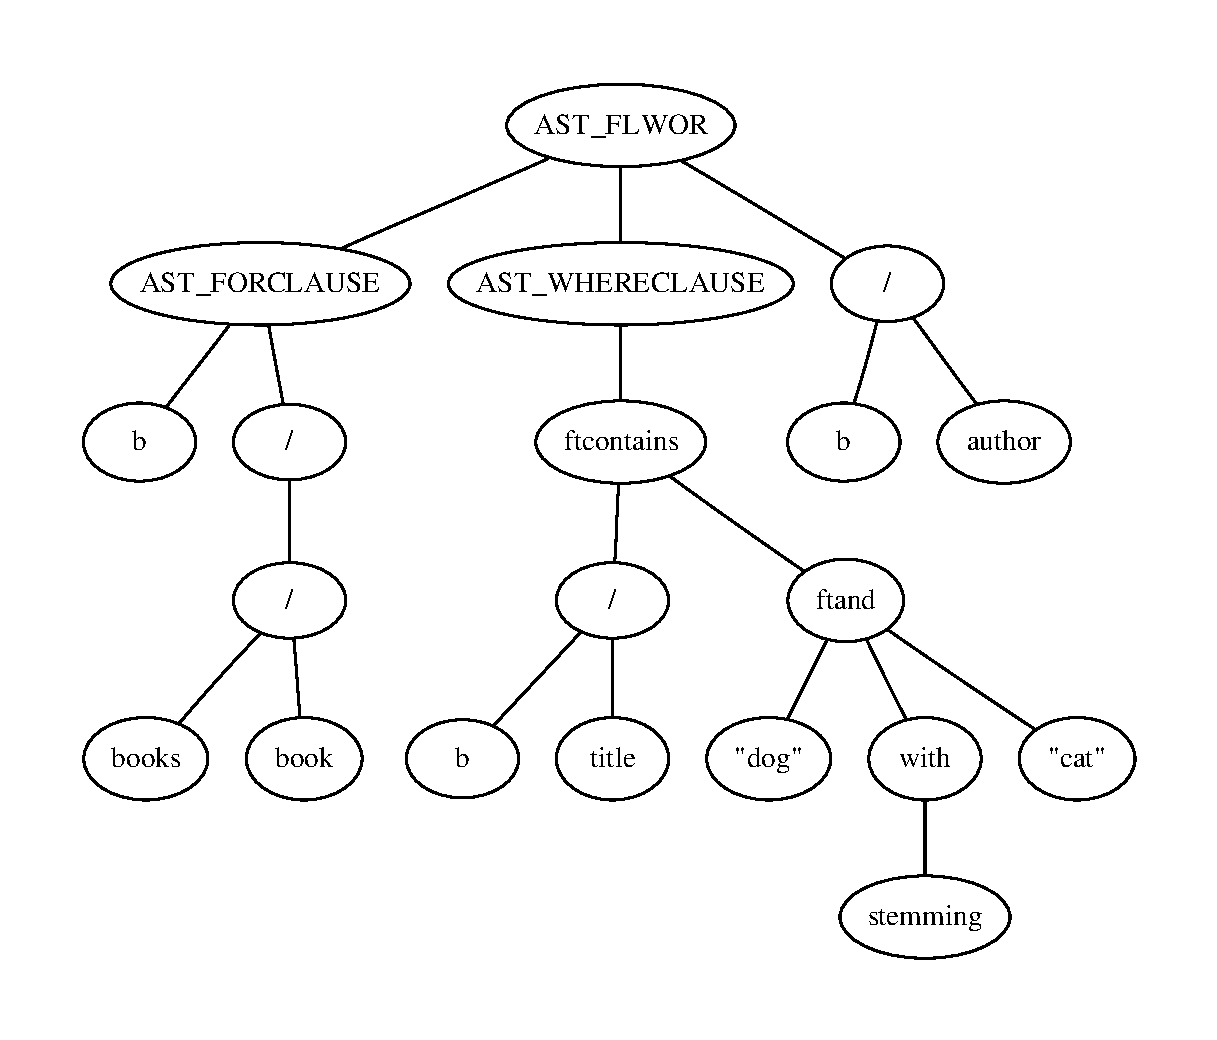
\includegraphics[scale=0.50]{img/graphs/ftq1} 
  \caption{Full-text query syntax tree}
  \label{figure:xquery:full_text_ast}
\end{figure}

\subsection{XQuery core}
\label{sect:theory:xquery:XQcore}
XQuery Core is a less powerful but semantically equivalent form of expressing
XQuery queries. XQuery Core as well as the process of normalizing regular
XQuery to XQuery Core is described in the document ``XQuery 1.0 and XPath 2.0
Formal Semantics''\cite{xquery_semantics}.

The goal of XQuery Core is to simplify queries and remove syntactic sugar,
leaving only the essential semantics without loss of expressiveness.
This is useful for optimization routines and translations into new types of
queries, for example relational algebra or SQL.

The process of normalization is described through a rich set of mapping
rules. These are documented in detail throughout ``XQuery 1.0 and XPath 2.0
Formal Semantics''\cite{xquery_semantics} and will not be reiterated here.
However we will examine some important examples.

First, however, it is important to take note of the syntax of the mapping
rules, as described in \cite{xquery_semantics}, section 3.2.2. 
 
\begin{figure}[!h]
  \centering
$
[Object]_{Subscript}, premises == Mapped Object
$
  \caption{Mapping rules syntax}
  \label{figure:xquery:mapping_rules}
\end{figure}

Consider figure \ref{figure:xquery:mapping_rules}. The left-hand side of the
equality symbol (==) denotes the original object to be rewritten. The
subscript indicates the type or kind of the object to be mapped, and/or
additional information to be passed between mapping rules. The right-hand side
denotes the rewritten object.

\subsubsection{Rewriting FLWOR expressions}
\label{sect:theory:xquery:core:rewriting_flwor}
\begin{figure}[!h]
\centering
[for $\$VarName_1$ $OptTypeDeclaration_1$ $OptPositionalVar_1$ in $Expr_1$,
\ldots, $\$VarName_n$ $OptTypeDeclaration_n$ $OptPositionalVar_n$ in $Expr_n$
$FormalReturnClause]_{Expr}$ \newline
$==$ \newline
for $\$VarName_1$ $OptTypeDeclaration_1$
$OptPositionalVar_1$ in $[Expr_1]_{Expr}$ return \ldots for $\$VarName_n$
$OptTypeDeclaration_n$ $OptPositionalVar_n$ in $[Expr_n]_{Expr}$ return
$[FormalReturnClause]_{Expr}$
  \caption{FLWOR expression mapping rule}
  \label{figure:xquery:flwor_mapping_rule}
\end{figure}

The mapping rule for FLWOR forclause-expressions can be seen in figure
\ref{figure:xquery:flwor_mapping_rule}. The mapping rule for LET expressions is
similar and omitted from this document for brevity, however they are also
normalized into several nested bindings.

\begin{figure}[!h]
\centering
$[where Expr_1 FormalReturnClause]_{Expr}$ \newline
$==$ \newline
$if ([Expr_1]_{Expr}) then [FormalReturnClause]_{Expr} else ()$
  \caption{Where-clause mapping rule}
  \label{figure:xquery:where_mapping_rule}
\end{figure}

\begin{figure}[!h]
\centering
$[stable? order by OrderSpecList FormalReturnClause]_{Expr}$ \newline
$==$ \newline
$[OrderSpecList]_{OrderSpecList} return [FormalReturnClause]_{Expr}$
  \caption{Order by clause mapping rule}
  \label{figure:xquery:orderby_mapping_rule}
\end{figure}

\begin{figure}[!h]
\centering
$[return Expr]_{Expr}$ \newline
$==$ \newline
$[Expr]_{Expr}$
  \caption{Return clause mapping rule}
  \label{figure:xquery:return_mapping_rule}
\end{figure}

Similarly, the mapping rules for where-clauses, orderby-clauses and
return-clauses can be seen in figures \ref{figure:xquery:where_mapping_rule},
\ref{figure:xquery:orderby_mapping_rule},
and \ref{figure:xquery:return_mapping_rule}.

For an example of how these rules are applied, consider the following FLWOR
expression:
\verbatiminput{graph_queries/flwor_rewrite1.xq}

By applying the mapping rules described,  this expression is typically
rewritten to:
\verbatiminput{graph_queries/flwor_rewrite2.xq}

The corresponding AST graphs can be seen in figures
\ref{tree:ast:flwor_rewrite1} and \ref{tree:ast:flwor_rewrite2}. In particular,
note that multiple for-clauses in a FLWOR expression is rewritten into several
nested FLWOR expressions, and that the where-clause is  rewritten into an
if-then-else expression. 

\begin{figure}[h!]
\centering
 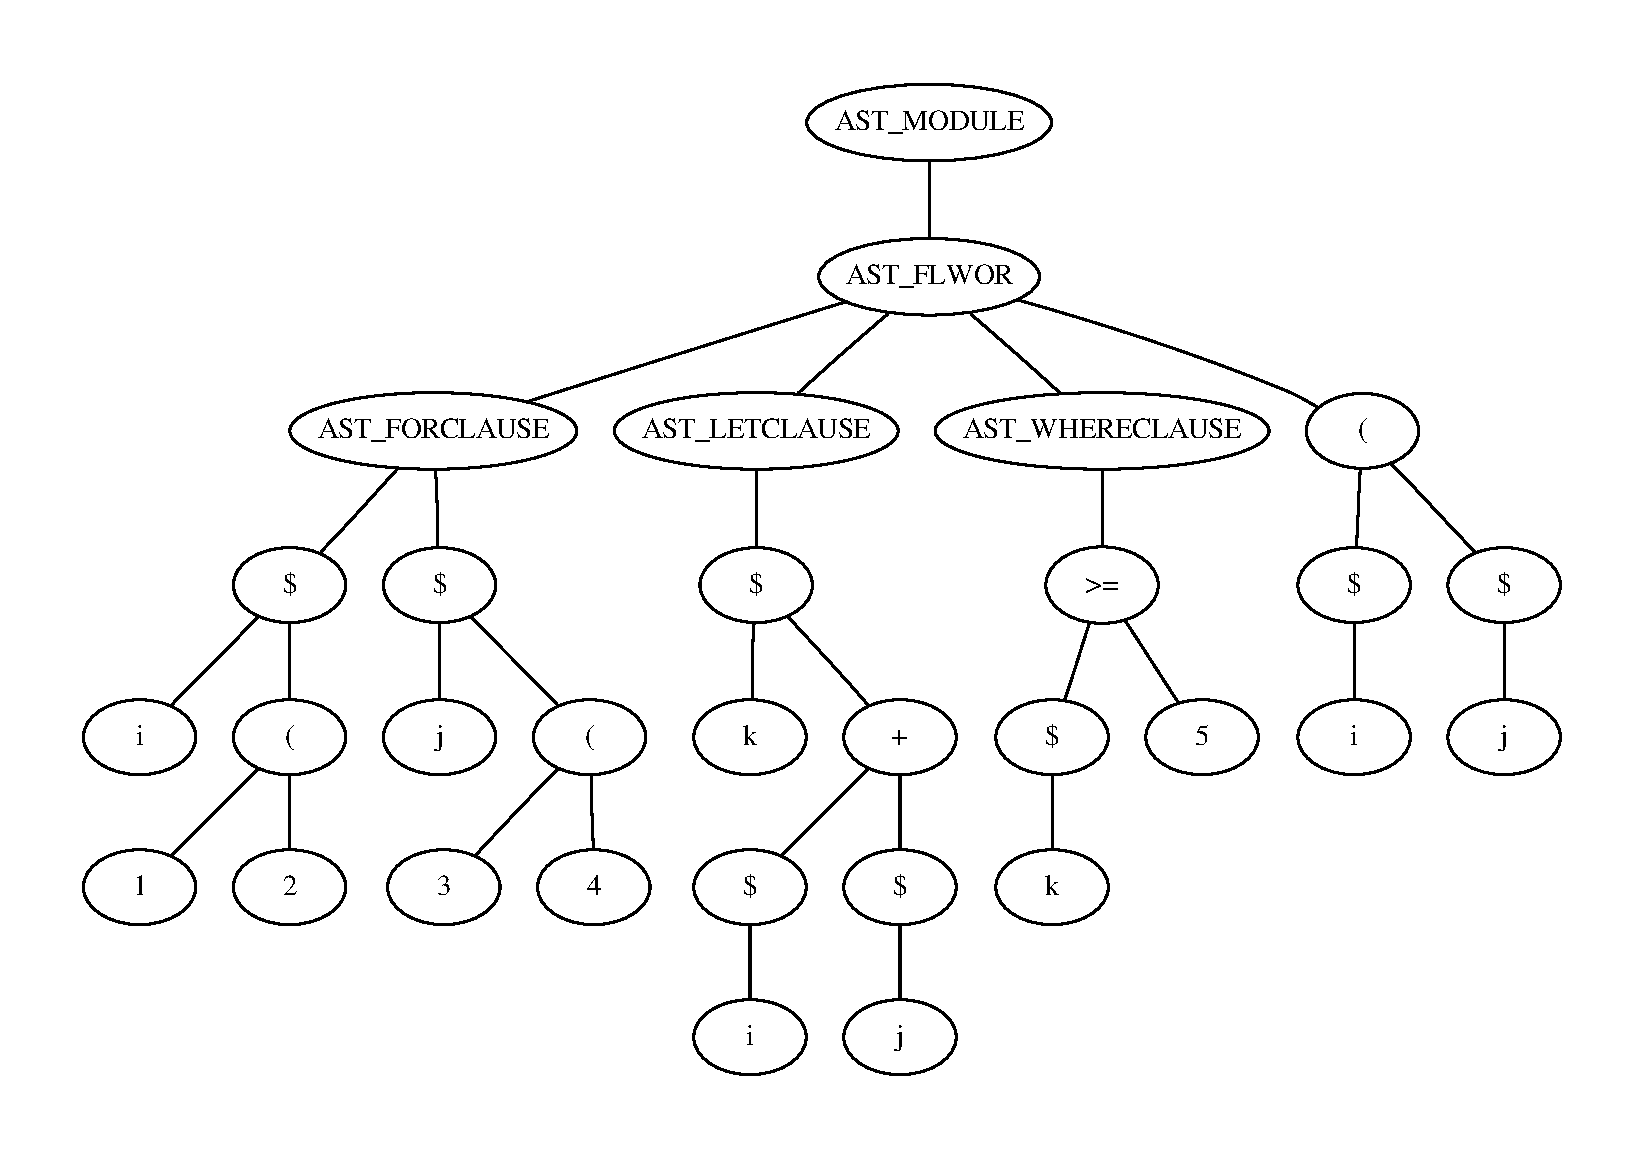
\includegraphics[scale=0.50]{img/graphs/flwor_rewrite1}
\caption{FLWOR AST tree before normalization}
\label{tree:ast:flwor_rewrite1}
\end{figure}

\begin{figure}[h!]
\centering
 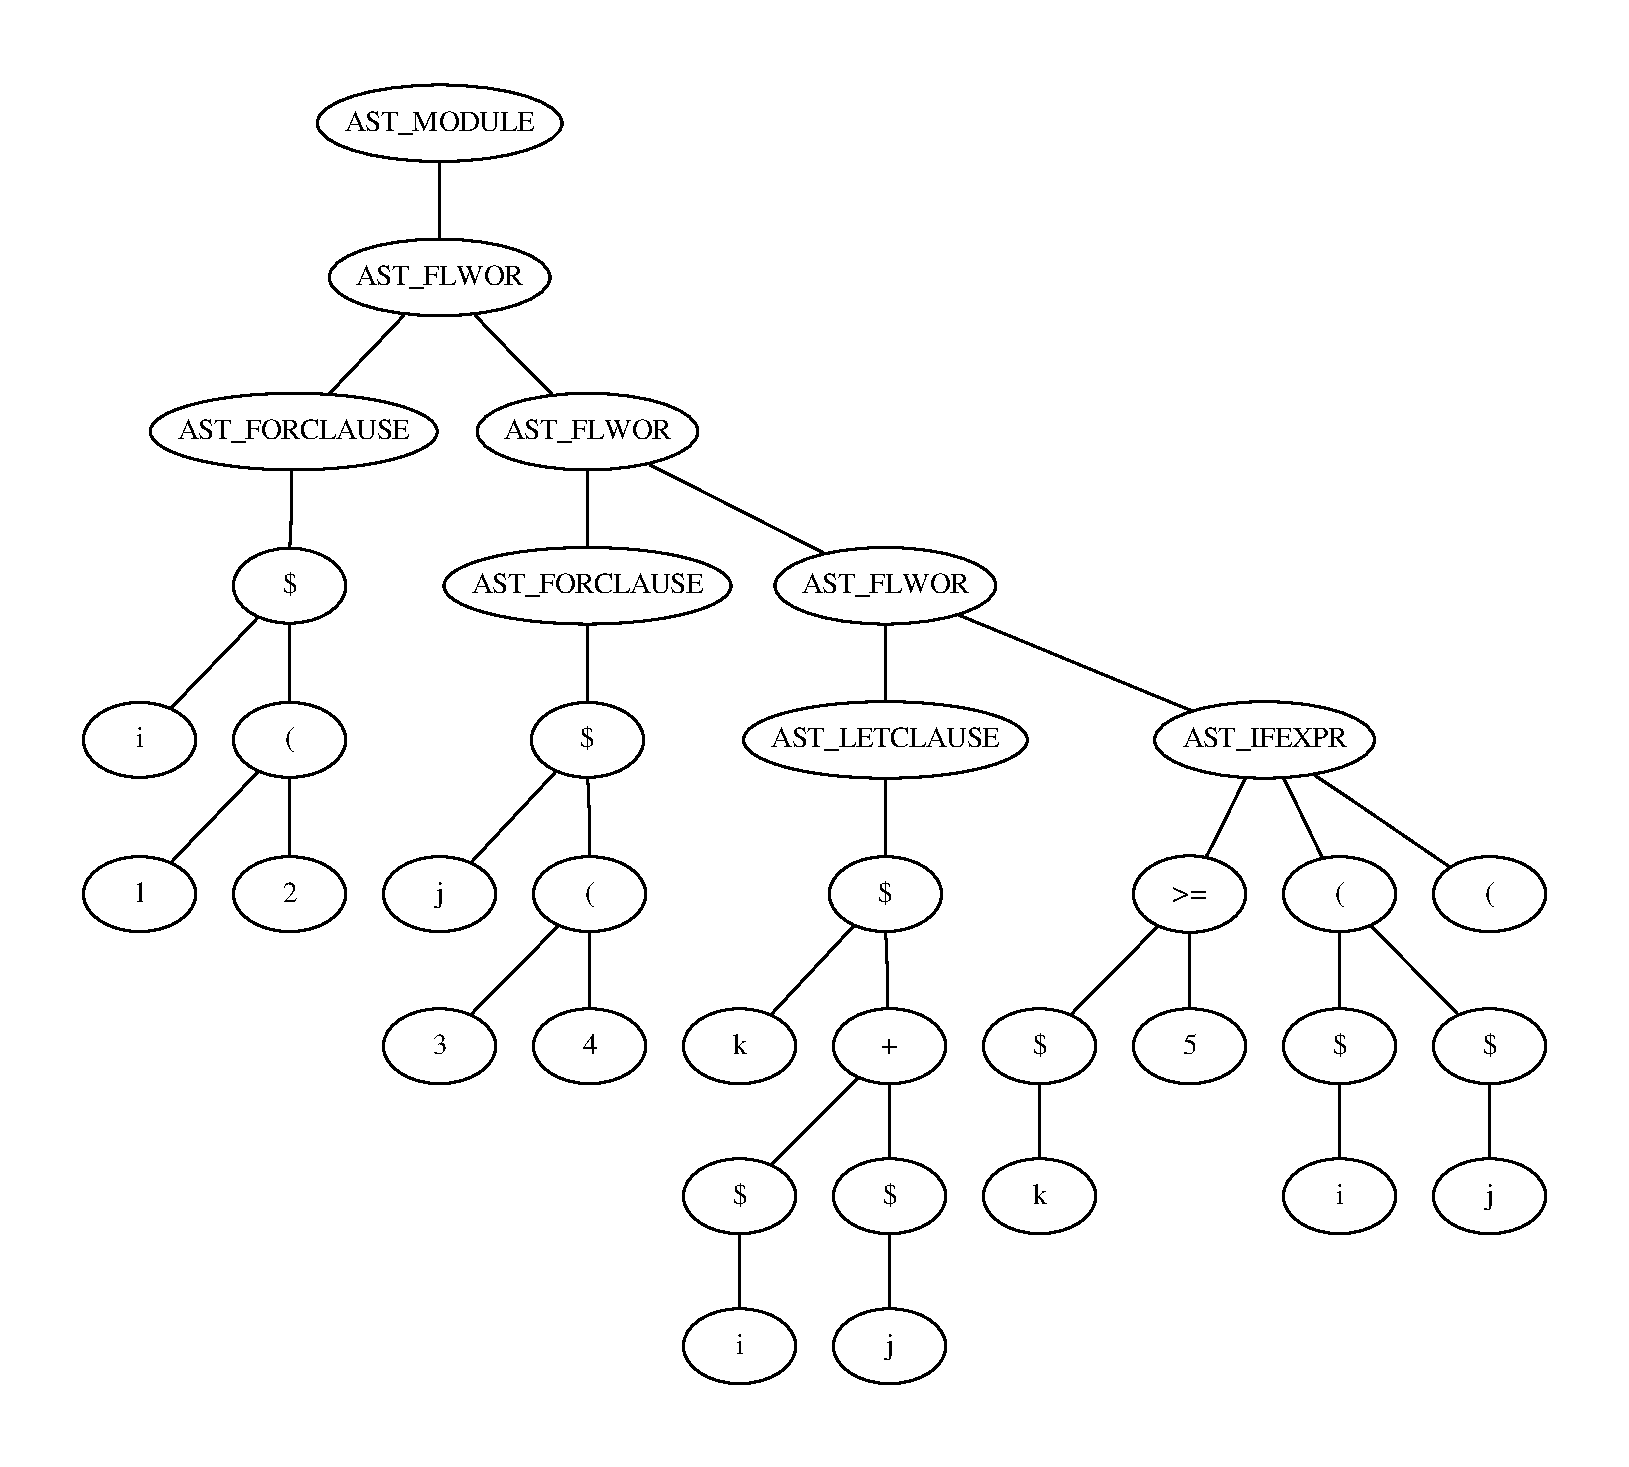
\includegraphics[scale=0.50]{img/graphs/flwor_rewrite2}
\caption{Normalized FLWOR AST tree}
\label{tree:ast:flwor_rewrite2}
\end{figure}

\subsubsection{Rewriting composite relative path expressions}
A composite relative path expression (for example, \verb!a/b!), can be
rewritten into a for loop using the mapping rule in
\ref{figure:xquery:relpath_mapping_rule}.

\begin{figure}[!h]
\centering
$[RelativePathExpr / StepExpr]_{Expr}$ \newline
$==$ \newline
fs:apply-ordering-mode ( \newline
fs:distinct-doc-order-or-atomic-sequence ( \newline
    let \$fs:sequence as node()* := $[RelativePathExpr]_{Expr}$ return \newline
    let \$fs:last := fn:count(\$fs:sequence) return \newline
    for \$fs:dot at \$fs:position in \$fs:sequence return \newline
       $[StepExpr]_{Expr}$
))
  \caption{Composite relative path expression mapping rule}
  \label{figure:xquery:relpath_mapping_rule}
\end{figure}

Given the trivial example \verb!a/b!, this translates into the following block
of normalized code:

\begin{verbatim}
fs:apply-ordering-mode (
fs:distinct-doc-order-or-atomic-sequence (
  let $fs:sequence as node()* := a return
  let $fs:last := fn:count($fs:sequence) return
  for $fs:dot at $fs:position in $fs:sequence return
    b))
\end{verbatim}

Which may seem like a rather verbose representation of such a simple path
expression. In particular, for complex path expressions this may
escalate into rather large rewritten expressions. However, this is a trade-off
to be made for normalization of such path expressions.

\subsection{AllMatches}
\label{sect:theory:xquery:allmatches}
\begin{itemize}
  \item http://www.w3.org/TR/xpath-full-text-10/\#AllMatchesSec
  \item Hva er AllMatches?
  \item Kobling til fulltekst
  \item Noen eksempler
  \item Den store forskjellen med AllMatches er at den minste enheten i et 
        dokument er et ord og ikke en tekstnode
\end{itemize}
\textbf{\underline{\LARGE TODO:}} Ikke sikkert at dette er noe poeng aa skrive
om hvis vi bare ignorerer fulltekst uansett. Kunne foreslaatt en tilnarming ala galatex kanskje, som bare
oversetter greiene til funksjonskall.
